\documentclass[a4paper,amsmath, 12pt]{article}

\pretolerance=10000

\oddsidemargin=1.0cm
\topmargin=-2.0cm
\textheight=725pt
\textwidth=390pt

\parskip=0.25cm
\parindent=0cm

\usepackage{color}
\usepackage{hyperref}
\usepackage{graphicx}% Include figure files
\usepackage[symbol]{footmisc}

%\pagestyle{empty}
\begin{document}


\begin{center}
\textbf{\Large Title of Your Article}

\vspace{0.5cm}

Author Name 1, Author Name 2,  Author Name 3 and Author Name 4 \footnote[1]{Corresponding author: Author Name 4, Centre for Mathematical Sciences, School of Engineering, Computing and Mathematics, University of Plymouth, PL4 8AA, UK. Email: firstnme.surname@plymouth.ac.uk.} \\

{\it Centre for Mathematical Sciences, \\ School of Engineering, Computing and Mathematics, \\ University of Plymouth, PL4 8AA}
\end{center}


\begin{abstract}
\noindent
Your brief abstract goes here. The abstract acts as a concise summary of your entire article. It should tell the reader what the report is about, in general terms. It should contain a skeleton
outline of,  the problem, what you have done, and your conclusions. 

%The abstract should not, if at all possible, use symbols or numbers, and should contain technical terms only if they are unavoidable and widely understood.

\end{abstract}


\section{Introduction}
This should describe the general context and background, including a general
description of what data are available, the manner in which and the purpose for
which they were collected.  It should also provide the aims of the investigation,
together with some indication of the methods used. It may well be an expanded
version of the summary.

Throughout your article, always properly quote any work you draw from other sources. This includes books (for example, \cite{james:2013} ), articles (for example, \cite{Seiichiro:2011}) and any other written resources you have used (for example, \cite{ONS}). \\

\section{Motivating Data}

Describe the data motivated your research. Give reference to where the data come from, what they are about, what have been collected and how they are relevant. Present and summarise the data.

\section{Methods}

Describe the methods underpinning your analysis. Methods should be described in a fair amount of detail. How much detail is always difficult to decide.  Aim to write as though for someone of comparable standing, e.g.  students who had done their second year and have recently started to learn about the project. The reader should be able to repeat the study on the basis of your report.

Formulae should be included as this is a statistical article, \textit{not} an essay. So please refrain from any ``subjective scientific writing''.

An equation is included as follows,
%
\begin{equation}
  X_i \sim N\left(\mu,\sigma^2\right), \, i = 1, \ldots, n, \, \mbox{independently},
\end{equation}
%
while two aligned equations would be:
%
\begin{eqnarray}
  y &=& b_0+b_1x \; , \\
  y &=& b_0+b_1x_1+b_2x_2 \; .
\end{eqnarray}
%
The format above (equations in extra lines) is called \textit{displaystyle}. If you write formulae within text, do not forget to enclose the maths expression in dollar symbols, e.g.\ like \verb|$a$|, which yields the maths letter $a$. This is proper maths  \textit{textstyle} --- I do not want to see just the ordinary letter ``a"!


Some additional maths typesetting rules are:
%
\begin{itemize}
\item Generally avoid font sizes that are too small. In particular, in textstyle write fractions in the form $a/b$ (rather than the ugly $\frac{a}{b}$).

\item Similar remarks apply to indices (powers, sub- and superscripts) in textstyle, in particular if they are more complicated expressions such as $x^{\frac{1}{1-x}}$.

\item Formulae should be treated as genuine parts of sentences, which includes the appropriate punctuation.
\end{itemize}



%\newpage %enforces new column here; normally NOT required




\section{Results}
In this section, give your results and interpret them. You may start with reporting the simple descriptive statistics. You will then report the results from your more advanced analyses.  Your interpretations should be expressed in a way that can be understood by non-statisticians. Try to interpret your results in the context of the application from which the data came.


\begin{figure}[h]
\begin{center}
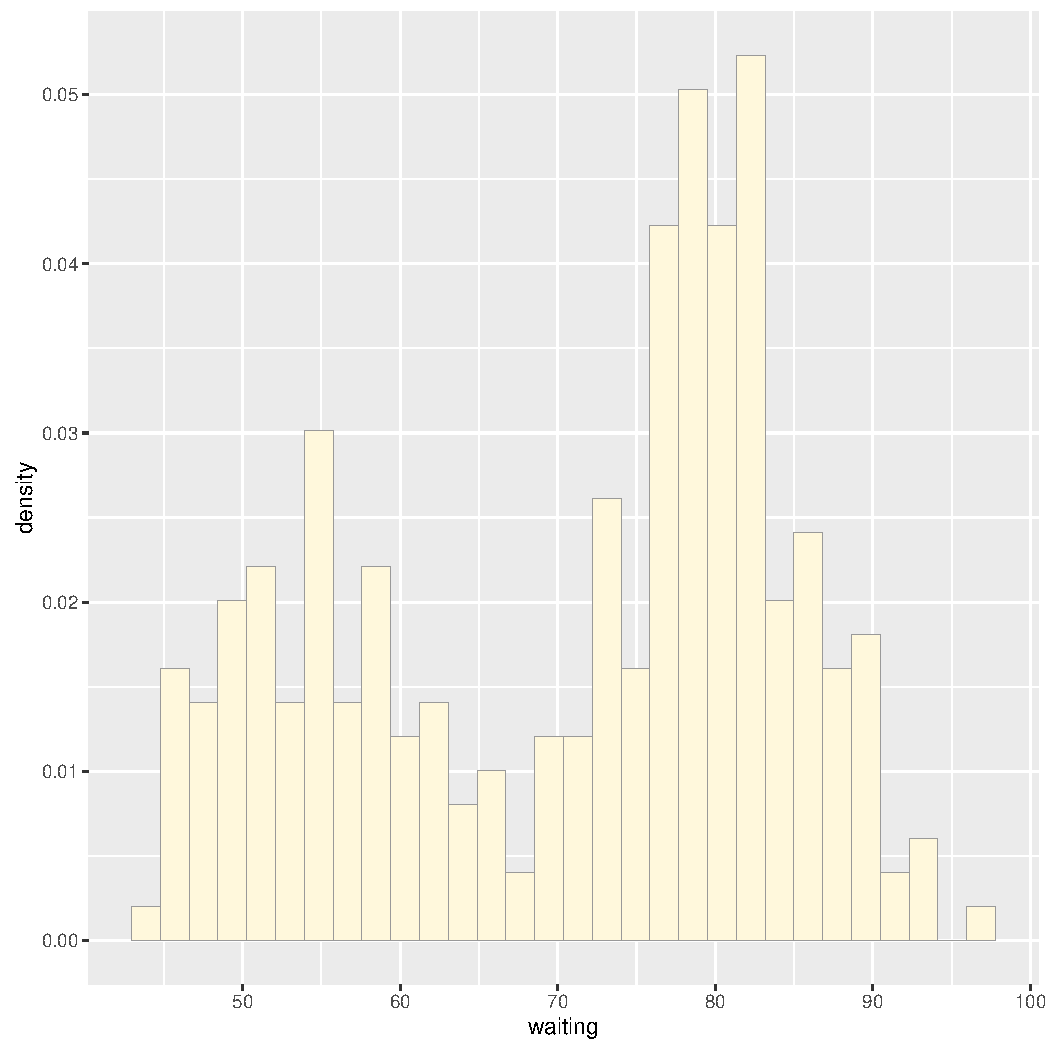
\includegraphics[scale=0.5]{figures/histogram.pdf}
\caption{\label{fig:hist} Waiting time between eruptions and the duration of the eruption for the Old Faithful geyser in Yellowstone National Park, Wyoming, USA.}
\end{center}
\end{figure}

Tables and graphs are useful tools to present your results. If you use pdflatex (recommended) you can include pdf pictures as shown for Fig.~\ref{fig:hist}.
Note that graph files should be in the same directory as the tex file (unless you prescribe the explicit path before the filename). Alternatively, you could use tables to report your results. Pay attention to the caption of your tables and figures. Good presentation means that readers can understand tables and figures in isolation without referring to the text.

If your article includes extensive results from real data analysis and/or simulation studies, try avoiding typing up the results manually. Instead, write R code to organise your results in tables which can be directly incorporated in your TEX file. Example R code which organises results into a TEX table can be found here: \href{https://github.com/Yinghui-Wei-team/copula-regression-models-semi-competing-risks/blob/main/data_analysis/table/table_hr.R}{example 1},
\href{https://github.com/Yinghui-Wei-team/copula-regression-models-semi-competing-risks/blob/main/data_analysis/table/table_reg_coef.R}{example 2},
\href{https://github.com/Yinghui-Wei-team/copula-regression-models-semi-competing-risks/blob/main/simulation_1_cox_underlying_copula/table/sim1_table.R}{example 3}, and \href{https://github.com/Yinghui-Wei-team/copula-regression-models-semi-competing-risks/blob/main/simulation_2_misspecifications/table/sim2_table.R}{example 4}.


\begin{table}[h]
\caption{A table}
\begin{center}
\begin{tabular}{|c|c|}
\hline
First Column & Second Column \\
\hline
1 & 2 \\
\hline
3 & 4 \\
\hline
\end{tabular}
\end{center}
\end{table}




\section{Discussion}

Summarise and discuss your findings. Provide an outlook to further work. It may be appropriate to give some account of previous investigation of the same or related problems, or to relate the present conclusion to others in a connected area. It is worth discussing how far the original aim was successfully achieved, if it was not, why not, and how you might have done things differently.

\vspace{1cm}
\textbf{Acknowledgments}

This research is funded by XXX (Ref: XXX XXX). Acknowledge funding body and give reference number.



\begin{thebibliography}{100}

\bibitem{james:2013}
J.~Gareth, D.~Witten, T.~Hastie and R.~Tibshirani, \textsl{An introduction to Statistical Learning with Applications in R}, Springer, New York, 2013.

\bibitem{Seiichiro:2011}
S.~ Morizawa, K.~ Shimoyama, S.~ Obayashi, K.~ Funamoto, and T.~ Hayase,
Implementation of visual data mining for unsteady blood flow field in an aortic aneurysm,
\textsl{Journal of Visualization"}, 2011, {\bf 14}(4), 393-398.

\bibitem{ONS} \url{http://www.ons.gov.uk/ons/rel/lifetables/interim-life-tables/2008-2010/sum-ilt-2008-10.html} (accessed 18-09-2016)

\end{thebibliography}



\end{document}
